\usetikzlibrary{arrows.meta}
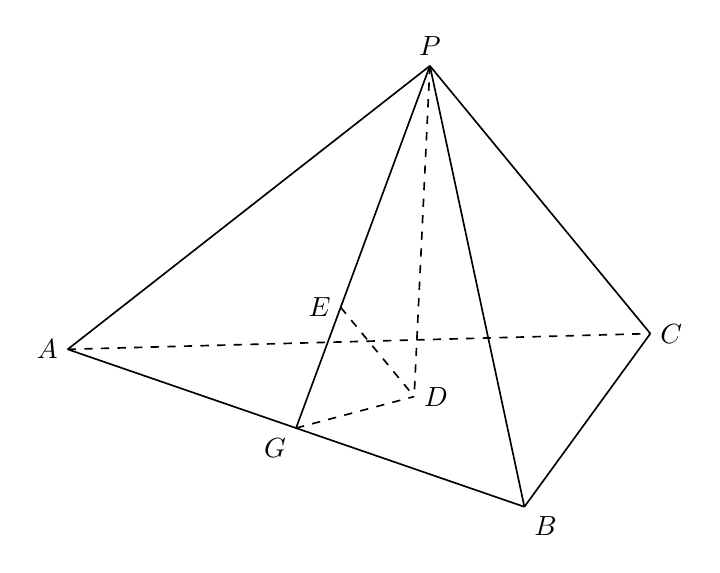
\begin{tikzpicture}[x=1cm,y=1cm,line width=.6pt,font=\normalsize,>=Stealth]
\coordinate (P) at (0.6,3.0);
\coordinate (A) at (-4,-0.6);
\coordinate (C) at (3.4,-0.4);
\coordinate (G) at (-1.1,-1.6);
\coordinate (B) at (1.8,-2.6);
\coordinate (D) at (0.4,-1.2);
\coordinate (E) at (-0.5333333333,-0.06666666667);
% base front edges (A-G-B collinear)
\draw[solid] (A)--(G);
\draw[solid] (G)--(B);
\draw[solid] (B)--(C);
% lateral edges
\draw[solid] (P)--(A);
\draw[solid] (P)--(G);
\draw[solid] (P)--(B);
\draw[solid] (P)--(C);
% hidden dashed edges
\draw[dashed] (A)--(C);
\draw[dashed] (P)--(D);
\draw[dashed] (G)--(D);
\draw[dashed] (E)--(D);
\node[above] at (P) {$P$};
\node[left] at (A) {$A$};
\node[right] at (C) {$C$};
\node[below left] at (G) {$G$};
\node[below right] at (B) {$B$};
\node[right] at (D) {$D$};
\node[left] at (E) {$E$};
\end{tikzpicture}
